\documentclass{article}
\usepackage[margin=3cm]{geometry}
\usepackage[utf8]{inputenc}
\usepackage{amsmath}
\usepackage{amssymb}
\usepackage{float}
\usepackage{enumitem}
\usepackage{graphicx}
\usepackage{caption}
\usepackage{subcaption}

\title{Nonlinear Optimization - Homework 1 }
\author{Christian Segercrantz 481056}

\begin{document}
	\maketitle
	\pagebreak
\section*{1.1}
	%First non-empty and convex
	%Theorem 2
	% ξ > (x − x) ≥ 0 for all x ∈ S
	We will first examine weather the set is non-empty and convex. We can see that the set is non-empty by finding a number that is contained in the set. Let us examine the point (1,1). The set is subject to $x_2 \geq x_1^2$ and $x_2 \leq 4$ and by inserting the point (1,1) into the conditions we get $1 \geq 1$ and $1 \leq 4$ which both hold. The set is thus non-empty.
	
%	By the definition of a convex function
%	$f(\lambda x_1 + (1 - \lambda)x_2 ) \leq \lambda f(x_1 ) + (1 - \lambda)f(x_2)$ we can examine wheater our function is convex. 
%	\begin{align}
%			((\lambda x_{1,1}+(1-\lambda)x_{2,1})-4)^2 + ((\lambda x_{1,2}+(1-\lambda)x_{2,2}) - 6)^2 & \leq \\
%			\lambda (( x_{1,1} - 4)^2 + ( x_{2,1} - 6)^2) + (1-\lambda) ((x_{2,1} - 4)^2 + (x_{2,2} - 6)^2) &
%	\end{align}
%Which we can see by solving analytically holds and the function is thus convex.
	From lecture 3, slide 3 we know that polynomial functions are convex functions. Since we have the sum of two second degree polynomial functions in different dimensions we can conclude that the function is convex. The epigraph of a convex function is also convex and the set is thus convex.
	
	The necessary optimality condition for our nonempty convex set is $\xi^\top (x -\bar{x}) \geq  0$. It is known that second degree functions are differentiable, and thus we know that $\xi = \nabla f(\bar{x})$. Thus the condition becomes
	\begin{equation}
		\nabla f(\bar{x})^\top (x -\bar{x}) \geq 0.
	\end{equation}
	The gradient becomes 
	\begin{equation}
		\nabla f(\bar{x}) = 
		\begin{bmatrix}
			2(\bar{x}_1-4) \\
			2(\bar{x}_2-6)
		\end{bmatrix}.
	\end{equation}
	The gradient at (2,4) becomes 
		\begin{equation}
		\nabla f(2,4) = 
		\begin{bmatrix}
			2(2-4) \\
			2(4-6)
		\end{bmatrix} =
		\begin{bmatrix}
			-4 \\
			-4
		\end{bmatrix} .
	\end{equation}
%	which means our expression becomes
%	\begin{align}
%		\begin{bmatrix}
%			2(\bar{x}_1-4) &
%			2(\bar{x}_2-6)
%		\end{bmatrix}
%		\left(\begin{bmatrix}
%			x_1 \\ x_2
%		\end{bmatrix} -
%		\begin{bmatrix}
%			\bar{x}_1 \\ \bar{x}_2
%		\end{bmatrix}\right)
%		& \geq 0. \\
%		\begin{bmatrix}
%			2(\bar{x}_1-4) &
%			2(\bar{x}_2-6)
%		\end{bmatrix}
%		\begin{bmatrix}
%			x_1-\bar{x}_1 \\ x_2-\bar{x}_2
%		\end{bmatrix}	& \geq 0. \\
%		2(\bar{x}_1-4)(x_1-\bar{x}_1) + 2(\bar{x}_2-6)(x_2-\bar{x}_2) & \geq 0 \\
%		2((\bar{x}_1 x_1 - \bar{x}_1^2 +4\bar{x}_1) + (\bar{x}_2 x_2 - \bar{x}_2^2 + 6\bar{x}_2 )) &\geq 0
%	\end{align}
	The complete expression then becomes 
	\begin{align}
		\nabla f(\bar{x})^\top (x -\bar{x}) &\geq 0 \\
			\begin{bmatrix}
			-4 &
			-4
		\end{bmatrix}
		\left(\begin{bmatrix}
			x_1 \\ x_2
		\end{bmatrix} -
		\begin{bmatrix}
			2 \\ 4
		\end{bmatrix}\right)
		& \geq 0 \\
		-4(x_1 - 2 + x_2 -4) = -4(x_1 + x_2 -6) & \geq 0
	\end{align}
	Due to our constraints of the function, choosing the largest possible values for x will result in the outcome $0\geq 0$ and any other value will result in a the LHS being greater than 0 since the parenthesis will be negative and the product, thus, result in a non-negative value. We have thus proven that the point (2,4) is optimal. Based on Theorem 1 in lecture 3, a optimal point of a convex function is a globally optimal point.

\section*{1.2}
	The closest point theorem says that $(x-\bar{x})^\top (x'-\bar{x})$ for any point x not in the convex set S and any point x' in the set S the point $\bar{x}$ is the closest point in the set S to y.
	Let's choose our point x' in the S to be $\bar{y}$ for x and $\bar{x}$ for y. Our two closest-point equations thus become
	\begin{equation}
		(x-\bar{x})^\top(\bar{y} - \bar{x}) \geq 0
	\end{equation}
	and
	\begin{equation}
		(y-\bar{y})^\top(\bar{x} - \bar{y}) \geq 0.
	\end{equation}
\section*{1.3}
	\subsection*{(a)}
		$a^\top x \geq \alpha$ and $a^\top x \geq \beta$ form half-spaces. Since $\alpha\leq\beta$ that are two options:
		\begin{enumerate}
			\item $\alpha = \beta \implies $ we have a hyperplane which is convex.
			\item $\alpha < \beta$ which is the area between two hyperplanes i.e. the intersection of half-spaces which is convex.
		\end{enumerate}	
		The set is thus convex.
	\subsection*{(b)}
		For a convex set it needs to hold that $\lambda x + (\lambda-1) y$
	\subsection*{(c)}
		The sets $a_1^\top x\leq b_1$ and $a_2^\top x\leq b_2$ form two half-spaces. Similarly part (a), there are two outcomes
		\begin{enumerate}
			\item The intersection of the half-spaces are empty $S=\emptyset$
			\item The intersection is non-empty $S\neq\emptyset$.
		\end{enumerate}
		A empty set is by definition convex. We know from exercise 2.1 we know that the intersection of convex sets are also convex. Since half-spaces are convex by lecture 2 slide 6 the set $S$ is convex.
	\subsection*{(d)}
		
\section*{1.4}
	\subsection*{(a)}
	Let us call $h(x) = Ax + b$.
	By lecture 3, slide 4 we know that that $f(x)$ is convex if $f(x) = g(h(x))$ if $g(x)$ is convex and $h(x)$ is affine. We can thus conclude that $f(x) = g(Ax+b)$
	\subsection*{(b)}
	Let $f(x)=\alpha h(x) + \beta$.
	By the definition of convex function we set
	\begin{equation}
		f(\lambda x + (1-\lambda) y ) =
		\alpha h(\lambda x + (1-\lambda) y ) + \beta.
	\end{equation}
	As we know that $h(x)$ is convex we can set
	\begin{align}
		\leq& \alpha (\lambda h(x) + (1-\lambda) h(y) ) + \beta \\
		= &\lambda \alpha h(x) + (1-\lambda)\alpha h(y) + \beta \\
		= & \lambda \alpha h(x) + \lambda\beta + (1-\lambda)\alpha h(y) + (1-\lambda)\beta \\
		=& \lambda (\alpha h(x) + \lambda) + (1-\lambda)(\alpha h(y) + \beta) \\
		=& \lambda f(x) + (1-\lambda)f(x)
	\end{align}
	Which proves that our function $f(x)$ is convex.
	\subsection*{(c)}
	Let $f(x) = e^{\beta x^\top A x}$ and A a positive semidefinite matrix $x^\top A x \geq 0$. Let $g(x)=e^x$ and $h(x)=\beta x^\top A x$. We know that $g(x)$ is a convex as per the lecture 3 slide 3. For a non-decreasing function it holds that $f'(x)\geq 0$. For $g(x)$ it means that $x\geq 0$.
	
	We can show that $h(x)$ is concave by showing that the Hessian of it is positive semidefinite, as per Theorem 12, lecture 3
	\begin{equation}
		H(h(x)) = \nabla^2 \beta x^\top A x = \beta 2 A
	\end{equation}
	We know that $\beta > 0$ and as stated before that the matrix A is positive semidefinite and thus the Hessian is positive semidefinite.
	
	By lecture 3 slide 4, we know that $g(h(x))$ is convex as long as $g(x)$ is a convex non-decreasing function and $h(x)$ is convex and positive-semidefinite. We have thus shown that $f(x) = e^{\beta x^\top A x}$ is convex.

\begin{figure}[H]
	\centering
	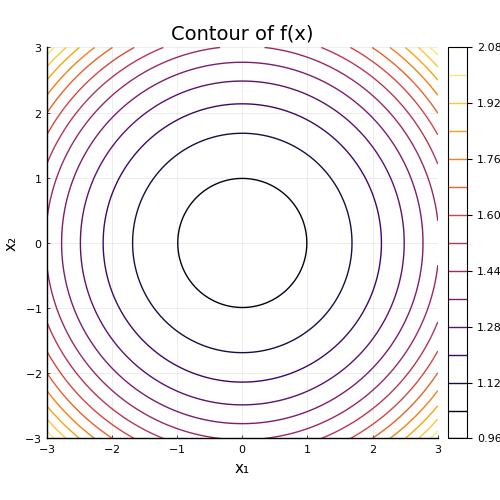
\includegraphics{plots/1_4c_contour.png}
	\caption{The contour plot of 1.4c}
	\label{fig:1.4c}
\end{figure}

\end{document}